\chapter{SELECTED MODEL ANALYSIS STUDIES\label{chapter:analysis_studies}}
The greatest benefit researchers receive from modeling is being able to reason about the uncertainty involved in observing a phenomena of choice.
From the modeling perspective, explicit statements about the uncertainty of a phenomena can be made by adding inputs to the model of the phenomena that represent a source of variance upon the phenomena.
In this section, I will introduce sensitivity analysis methods that I adapt to use in the SMS pipeline as a method for identifying how uncertainty in input variables impacts our uncertainty in output variables within the uniform SMS representation.
Once introduced I will show how the outputs from sensitivity analysis can be used to inform other methods of model analysis, both automatic methods and ones that can be used interactively by the domain modeler.

\section{Structural Model Analysis\label{sec:structural_analysis}}

\subsection{Overlap Identification\label{sec:overlap_identification}}
While analytical methods can provide a large amount of useful information to modelers about a single model, the real benefit of the AutoMATES system comes from the ability to automate comparisons among competing models. Competing models can be identified from the output variables of their computation graphs. After identifying a selection of competing models the comparison phase can begin.

For any two competing models of the same phenomena the comparison phase consists of the following:

\begin{enumerate}
  \item Identify the overlap between the variables in each models computation graphs. This corresponds to overlap in observable real-world phenomena.
  \item Extract the sub computation graphs for each model based on the variable node overlap.
  \item Perform analysis on the overlapping computation graphs and compare the results with the analysis results from the models whole computation graphs.
\end{enumerate}

In order to accomplish the tasks outlined above, I will introduce a new construct, known as a Forward Influence Blanket (FIB). A FIB is a specific instance of a Markov blanket \citep{pearl2009causality}, derived from a GrFN computation graph, that can be used for forward analysis.  % TODO: possibly define forward analysis and markov blanket
After the completion of these tasks the information gained from the comparative study of these models can be added to the final model report, or used for automatic model selection. In this chapter I discuss model comparison in terms of two models compared directly with one another. At the end of the chapter I will elucidate on the necessary steps to generalize this form of binary model comparison to a set of $N$ models.

\subsubsection{Identifying a Forward Influence Blanket\label{sec:fib_creation}}
Imagine the structure of two computational models of the same phenomena in the most general sense. We can say with certainty that both models will have the same output variable, namely the variable that represents the phenomena of interest. From this there are three options for how the set of input variables between the two computational graphs can overlap. The least interesting option is that the two models could share no inputs variables. This would mean that the computations involved in each model are wholly independent and could be combined if necessary in a trivial manner, at least at the input level. The more interesting option is that a subset of the inputs are shared between the two models. This entails that the models will make use of the same data, though the computations used to transform that data into a model output will almost certainly differ. It is possible that the set of input variables will overlap exactly between the two models; however, it is much more likely that there will be some input variables that are not contained in both. In the following subsections I will discuss how to build a computation graph that represents the computation present in a GrFN that corresponds to utilization of shared variable nodes with another model.

% TODO: Add material about Shared Structure Identification here
The shared structure components of a FIB for two models of the same phenomena are identified using the following strategy.
By definition the models share the same output variable node.
Therefore any shared structure will be within the range of a shared variable node, either an input variable or an inner variable node, and all the full computation path to the output node.
A set of shared nodes between the two graphs can be discovered using node name matching on the grounded node names.
This is done upon the CAG view of the GrFN CG so that variable nodes are only matched once and not once per update recorded in the overall CG.
Using the set of shared nodes and the output node we can discover all computation paths that lead to the output node by doing an exhaustive path search from each shared node to the output node \citep{sedgewick2002algorithmsInC}.
Combining the outputs from all of these paths together gives us the shared portions of each GrFN CG that serve as the basis for each models FIB.

% TODO: The section discusses Cover Set Variables
The key aspect of a FIB that distinguishes it from a GrFN computation graph is that the portions of the original computation graph that are not shared between the two models under comparison are pruned.
In order to ensure that the resulting models are still executable, variable nodes representing new inputs to the FIB computation graph must be retained.
This set of variables has been identified as the cover set.
Forming this cover set and adding it to the shared overlap portion of each GrFN CG as mentioned above is the last step necessary to fully create the FIB for each model.
Identifying a variable as being a member of the cover set stems from the initial shared graph structure extracted from the original GrFN CGs.
All nodes along the shared structure must be compared to the node structure in the original CG.
If any nodes are missing a branch that is present in the original CG then the immediate parent of the node must be added to the set of cover nodes and is grafted on to the FIB.
Once the set of cover nodes are added to the shared graph structure the FIBs for each model are complete.
To visualize what a FIB looks like for both a small and large CG we have added the FIBs that denote the overlap between the two evapo-transpiration models.

\FloatBarrier
\begin{figure}[!tbp]
  \centering
  \subfloat[PETPT FIB CAG]{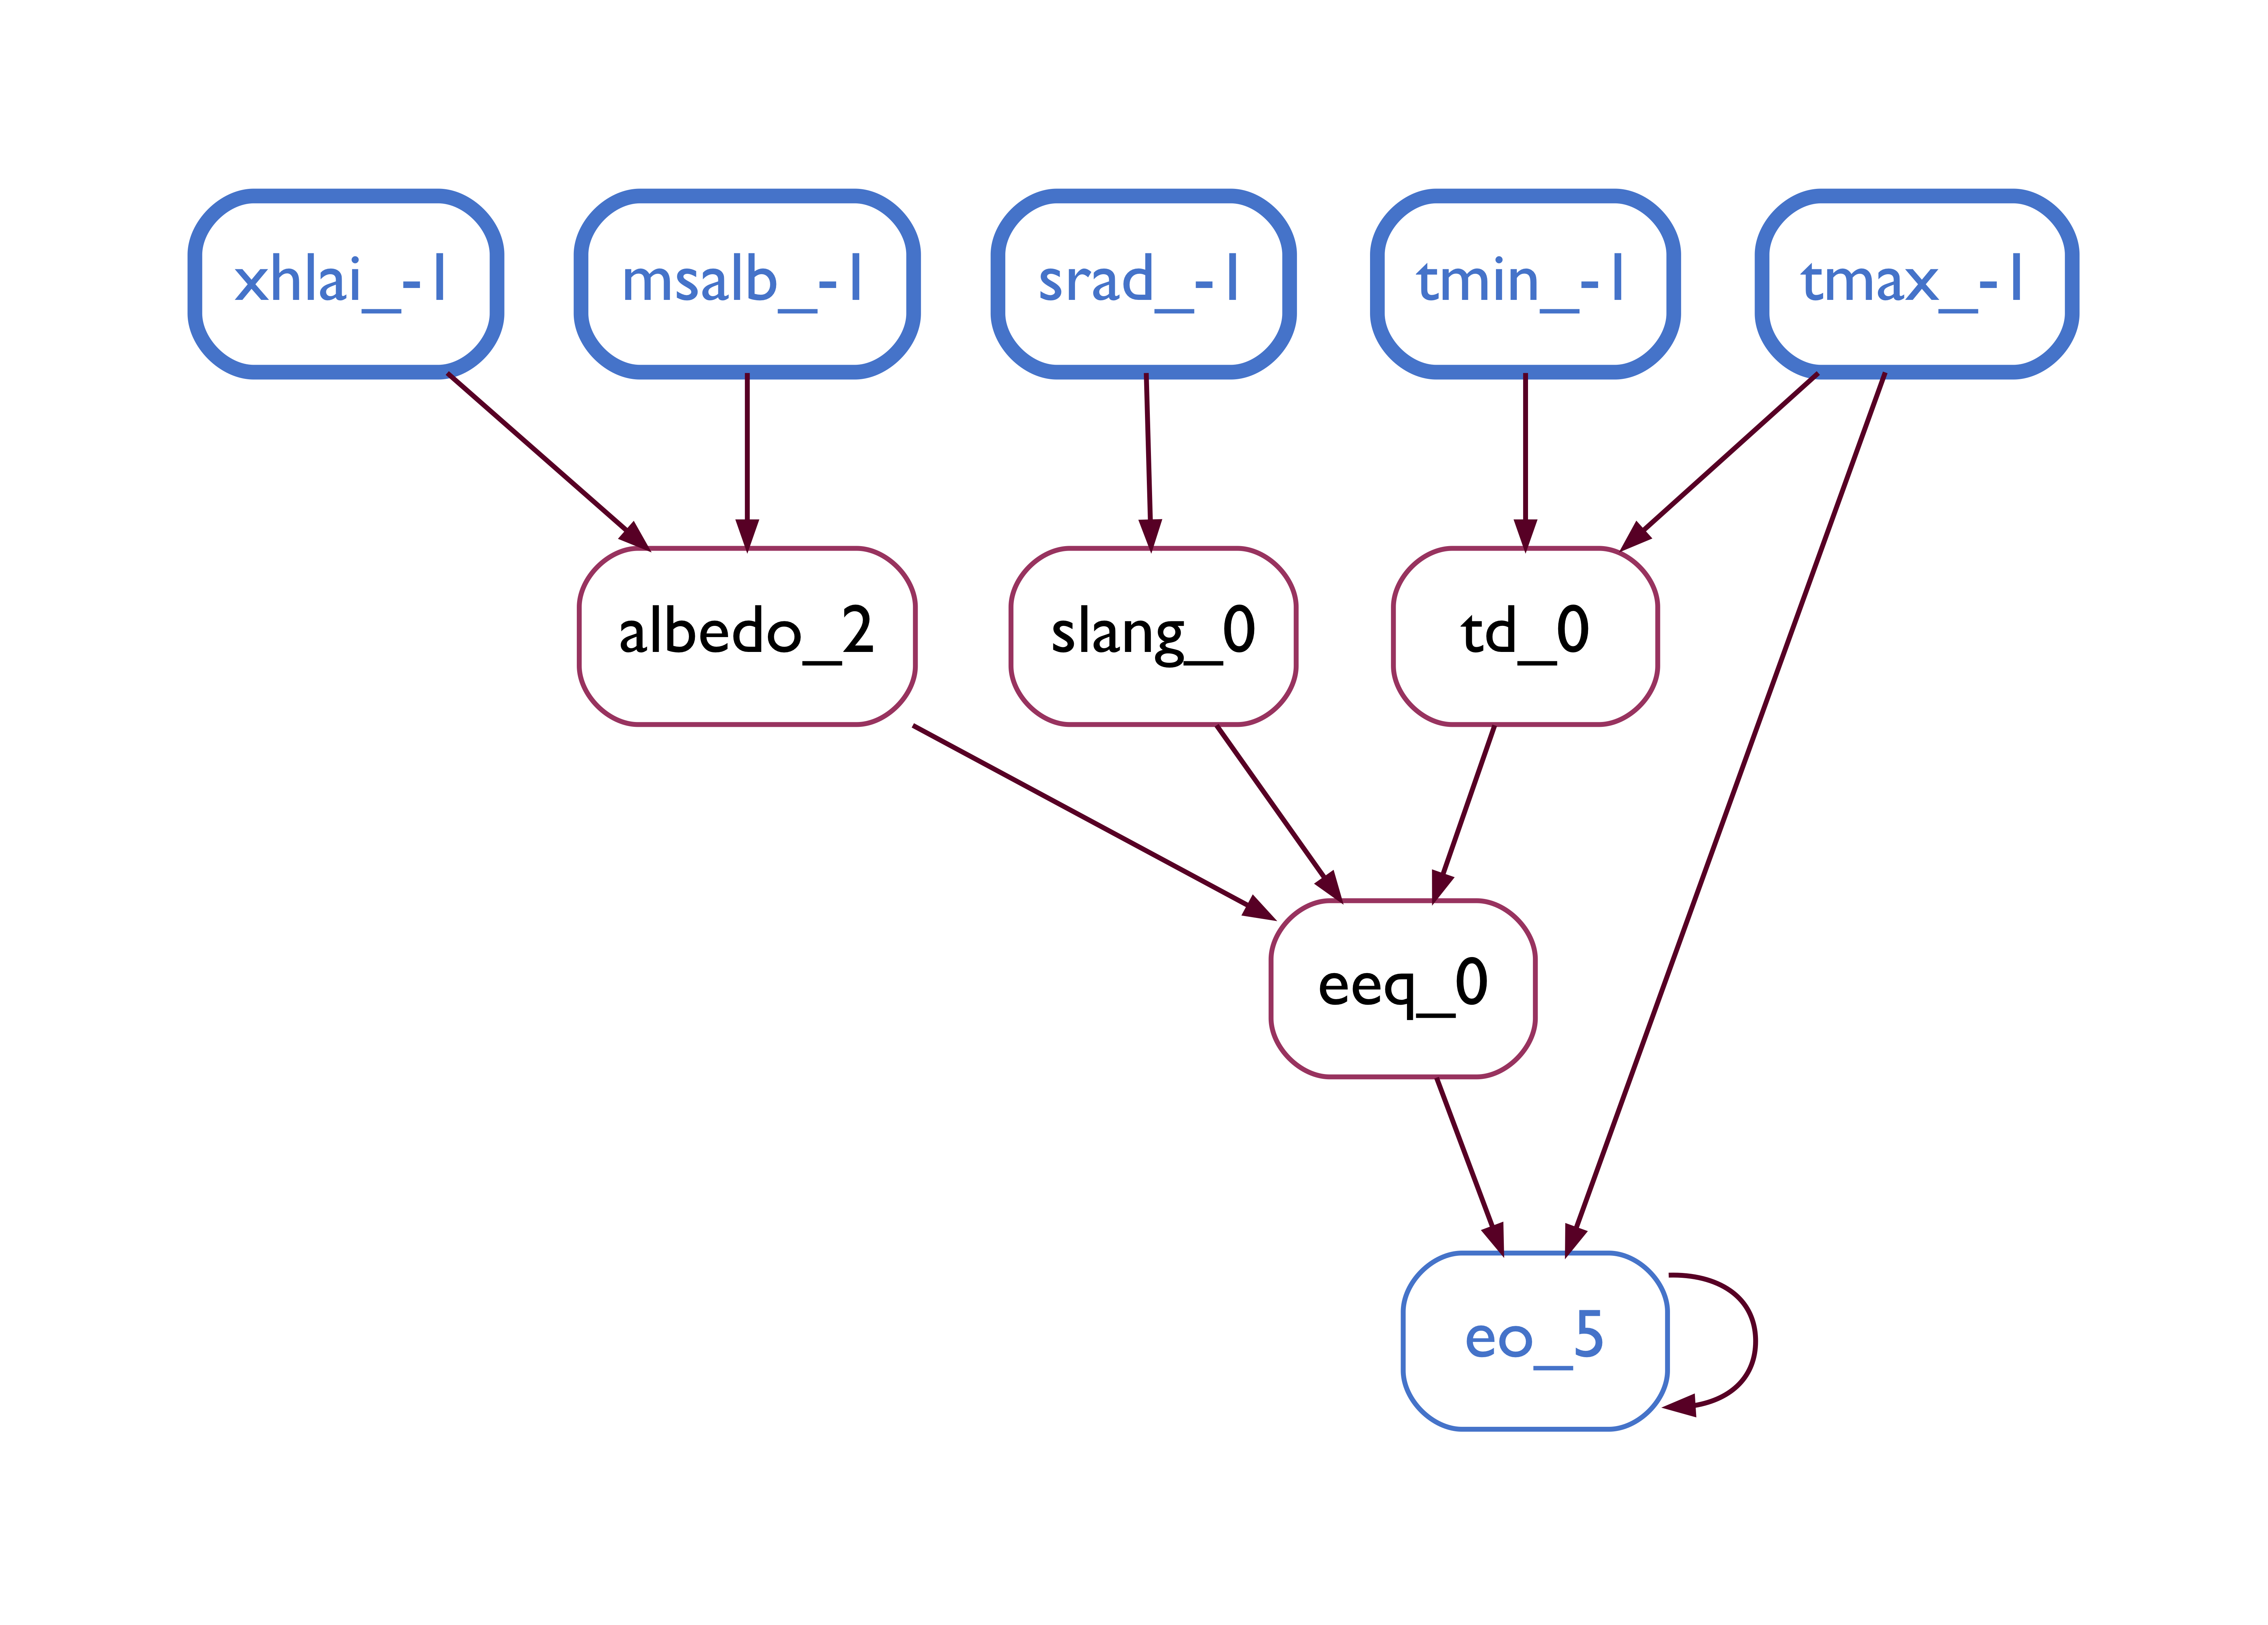
\includegraphics[width=0.75\textwidth]{PETPT_FIB_CAG}\label{fig:petpt_fib}}

  \subfloat[PETASCE FIB CAG]{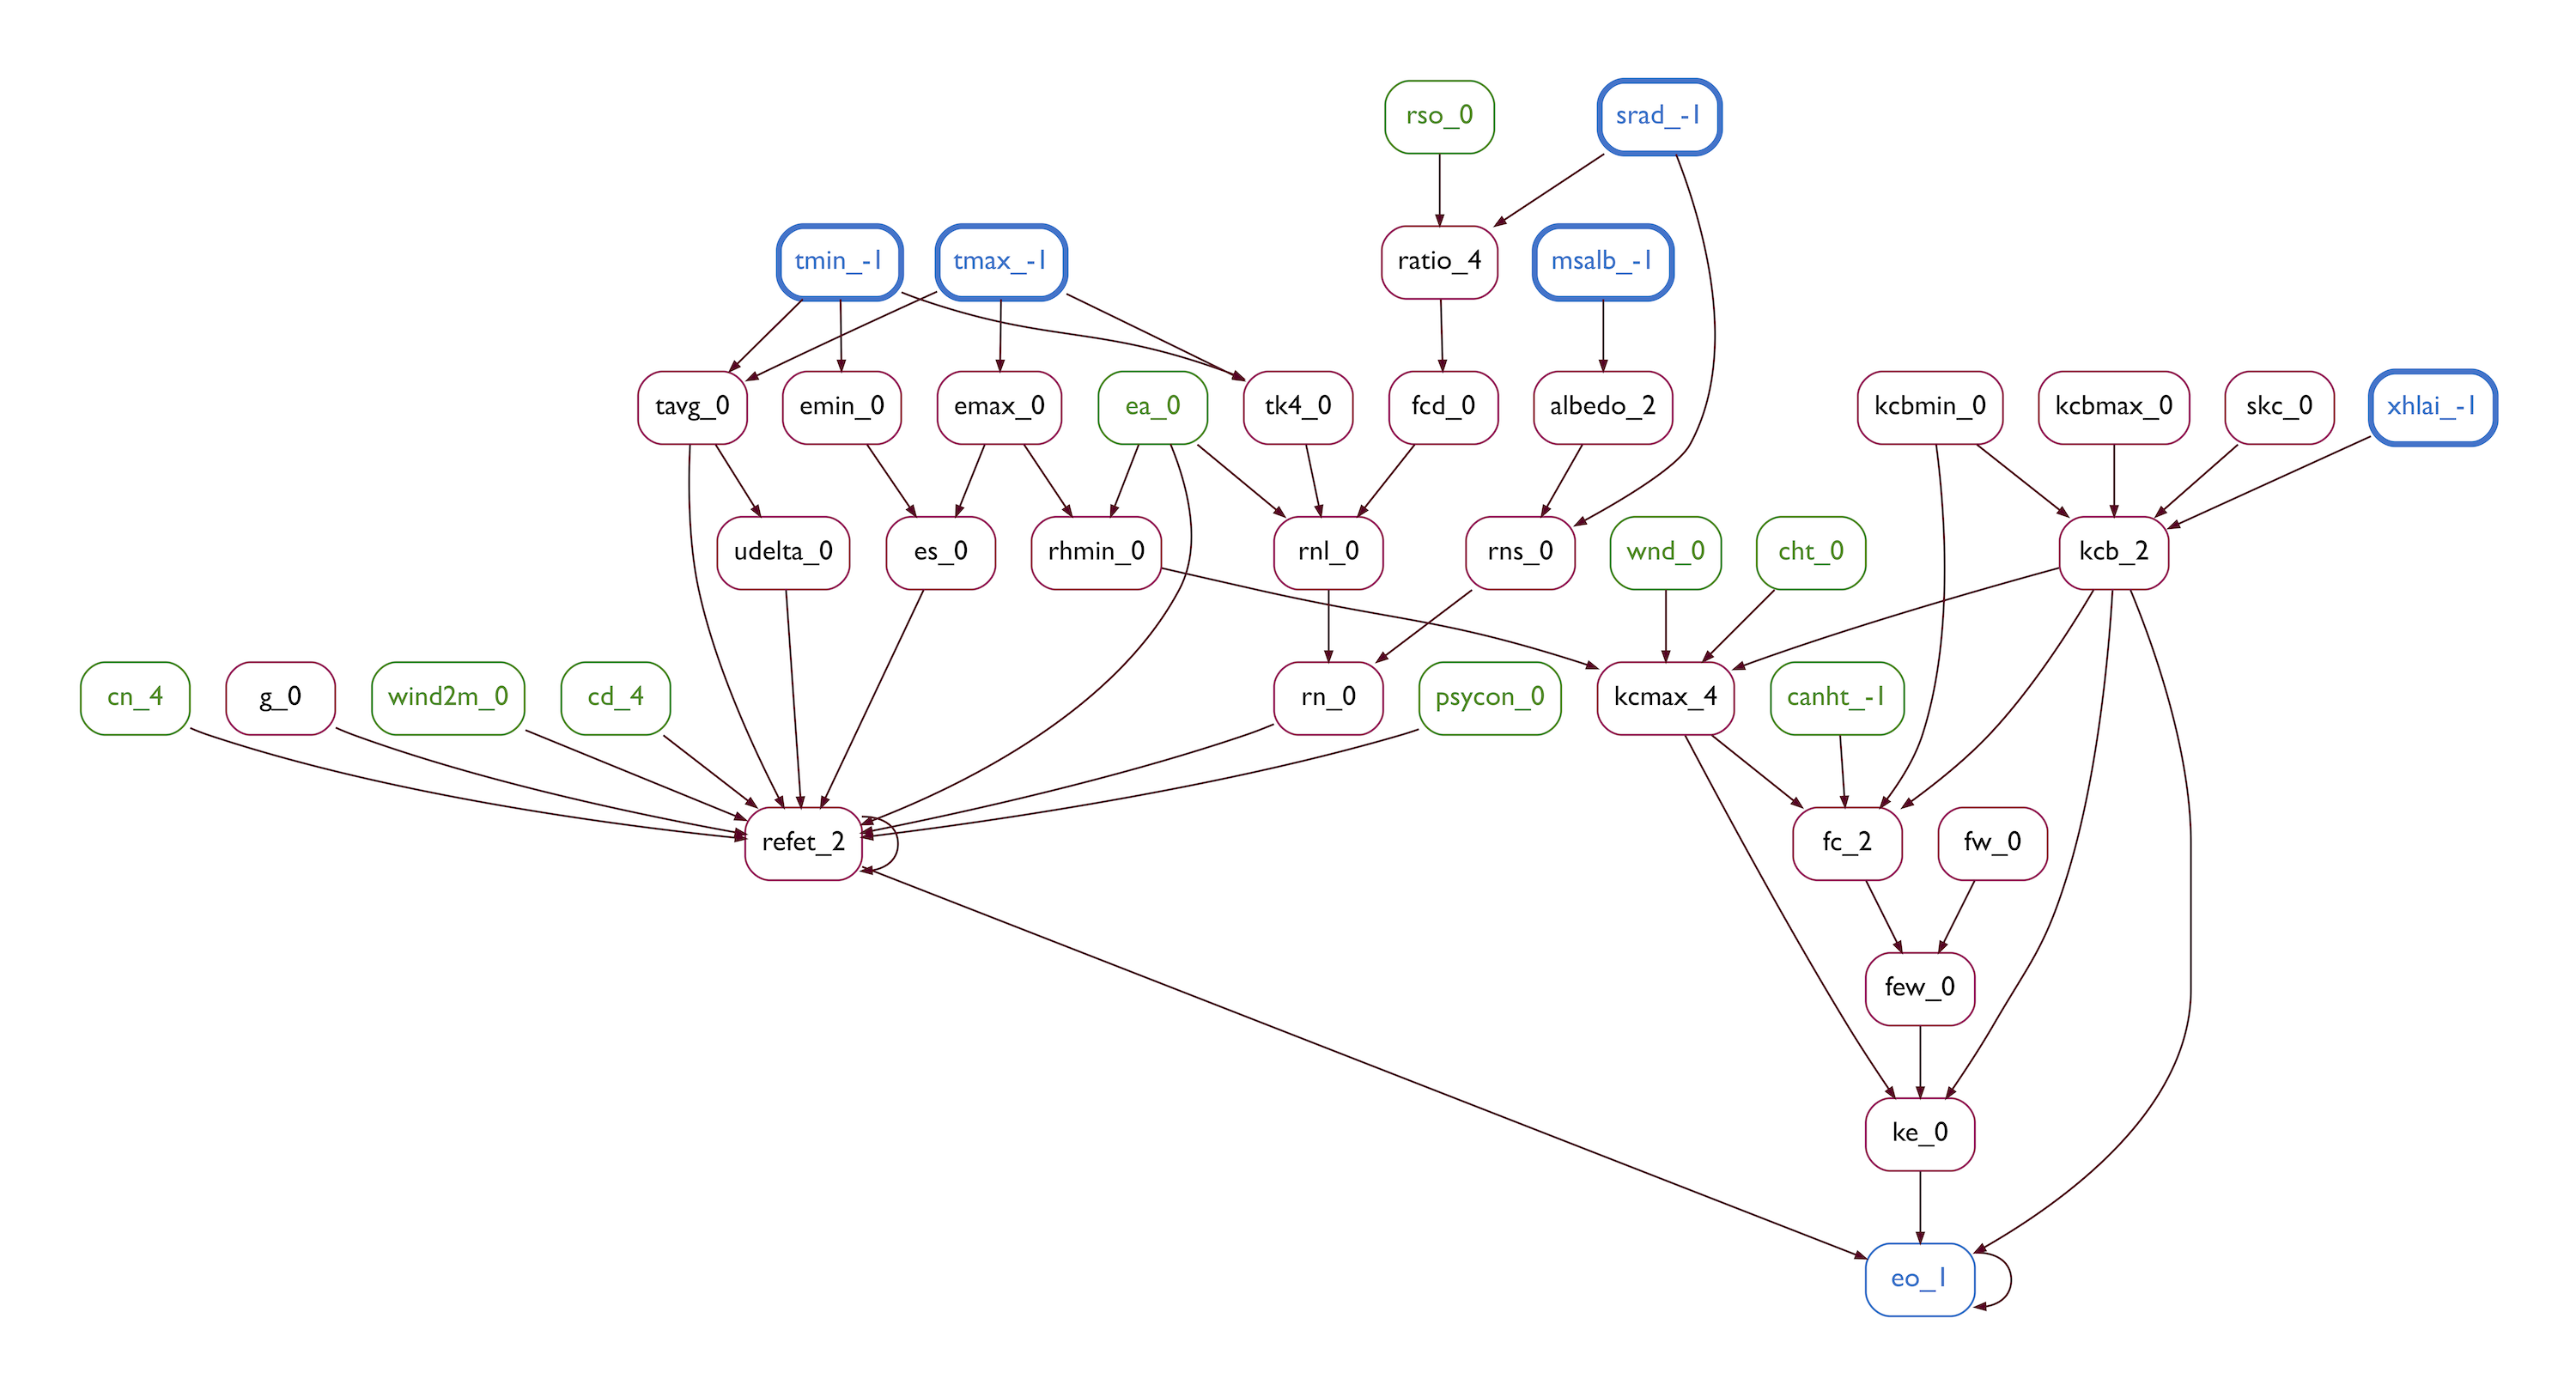
\includegraphics[width=0.75\textwidth]{PETASCE_FIB_CAG_smaller}\label{fig:petasce_fib}}
  \caption[Forward Influence Blanket CAG Examples]{Forward Influence Blanket (FIB) CAGs for the PETPT and PETASCE evapo-transpiration models that depicts the overlap with each other. Note that shared variables are shaded in blue and shared input variables are both shaded blue and bolded. Note that while the PETPT model did not have any variable nodes in the cover set the PETASCE model has several variables in the cover set. These variables are shaded green.}
\end{figure}
\FloatBarrier

\subsubsection{Input Set Execution on a FIB\label{sec:fib_exec}}
In order to execute a FIB the user must provide values for the input variable nodes and values for the cover variable nodes. At execution time, both sets of variable nodes will be populated before beginning to compute the function nodes in the partial order of functions provided by the GrFN computation graph. This is the only difference between computing on a FIB computation graph and computing on a GrFN computation graph.

Execution of a FIB computation graph can be done either with singular preset values for all of the cover variables, or with ranges for each cover variable.
FIB CGs support Torch-aided vectorized computation similar to the GrFN CG structure, and no additional memory constraints are imposed on execution by the FIB class.

\section{Functional Model Analysis\label{sec:functional_analysis}}

\subsection{Global Sensitivity Analysis\label{sec:sens_analysis}}
A powerful tool used by modelers to quantify the uncertainty present in models is global sensitivity analysis. Broadly speaking, global sensitivity analysis is the study of how variance in the inputs of a model affect the variance, or uncertainty in the output of the model. Since the goal of the SMS pipeline is to provide modelers with a tool select a model that lowers the amount of uncertainty in estimation of a given phenomena we have chosen to use sensitivity analysis in order to evaluate the extracted models.

For this thesis we employ variance-based methods of sensitivity analysis.
% TODO: give a good definition of variational methods of sensitivity analysis
Variance-based methods of sensitivity analysis focus on the computation of sensitivity indices. Sensitivity indices are numerical values assigned to each model input, or set of inputs, that denote how sensitive the output of the model is to that input, or set of inputs. The first order sensitivity index, commonly denoted by $S_1$, notates the sensitivity of the model output from each individual input. Similarly the second order sensitivity index, commonly denoted $S_2$, notates the sensitivity of the model output from each pair of model inputs. This pattern continues for any given model for all higher order sensitivity indices.
The final sensitivity index is the total sensitivity index, commonly denoted as $S_T$. This index has an entry that corresponds to each model input. Each entry tracks the total amount of sensitivity on the model output contributed by the input as a portion of the first, second, and all higher order sensitivity indices.

While other methods of sensitivity analysis exist, such as Variogram Analysis of Response Surfaces (VARS), the variance-based methods fit well within the scope of our problem domain as we are conducting sensitivity analysis over probabilisitic models.
While the VARS method does claim a significant faster computation time, it does not reveal as much information about the affects of model inputs upon the model output.
This is due to the lack of pairwise-information that the variance-based methods are able to capture.
In the following subsections I will discuss Sobol analysis, developed by \citet{sobol2001globalSA}, that will be used to perform variance-based sensitivity analysis upon the extract scientific models and I will address how it has been adapted for use by the SMS pipeline.

\subsubsection{Sampling Inputs with the Sobol Sequence\label{sec:sobol_seq}}
Sobol analysis is the most widely used version of variance-based sensitivity analysis. The Sobol analysis method gets its name from the sampling method used during analysis. Samples for Sobol analysis are drawn from the Sobol sequence. Defining the precise nature of the Sobol sequence is beyond the scope of this masters thesis; however, we can observe how the Sobol sequence aids sensitivity analysis by observing the differences between draws from the Sobol sequence and draws from a random sample. A visualization of the difference is shown below in figure \ref{fig:sobol_seq_vis}.

\FloatBarrier
\begin{figure}[!htbp]
    \label{fig:sobol_seq_vis}
    \centering
    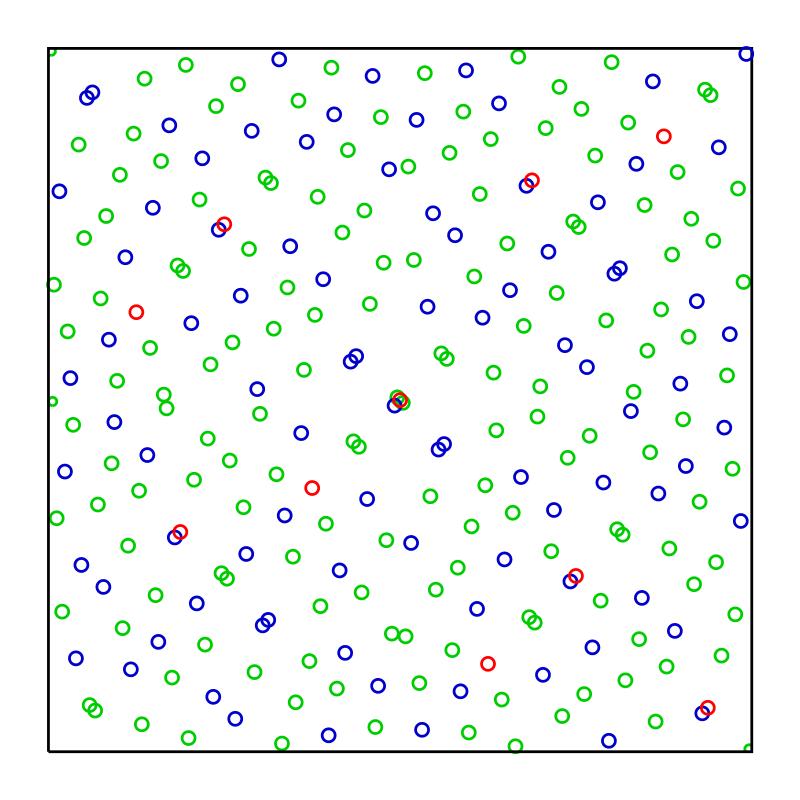
\includegraphics[width=.45\textwidth]{sobol_samples}\hfill
    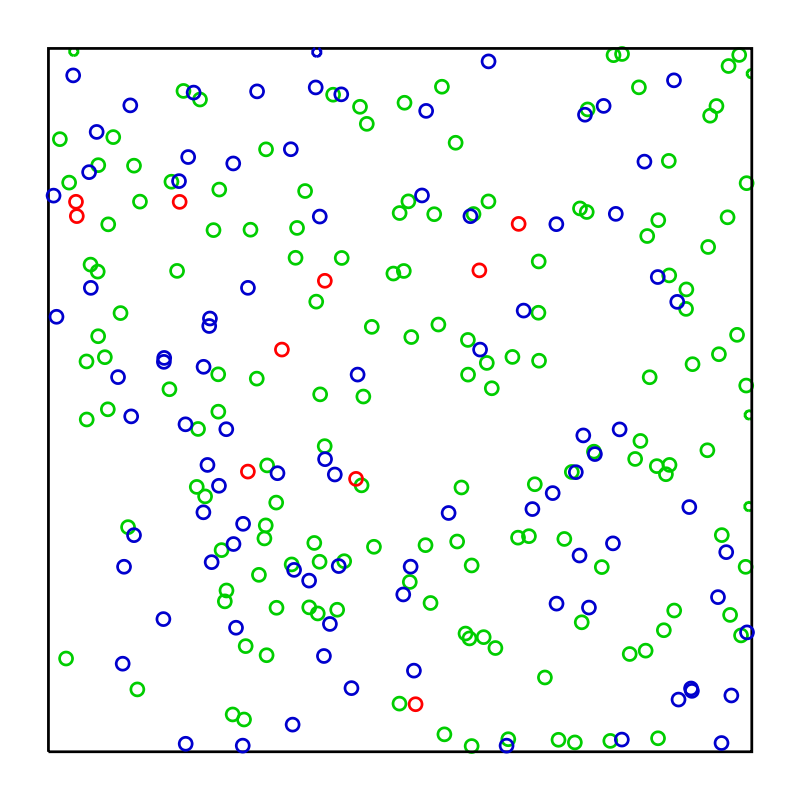
\includegraphics[width=.45\textwidth]{random_samples}
    \caption[Sobol Sequence Visualization]{A visualization of 1000 draws from the Sobol Sequence (left) paired with 1000 randomly drawn points (right) in two dimensions. For both images the first 10 draws are colored red, the remaining first 100 draws are colored blue, and the remaining 1000 draws are colored green. Images created by James Heald, distributed under a CC BY-SA 3.0 license.}
\end{figure}
\FloatBarrier

Notice that the red, blue, and green draws from the Sobol sequence are much more evenly dispersed across the sample space than the same draws from a uniform random sample. This allows the Sobol sampling method to achieve much better coverage of the search space, while still maintaining some variability in sample locations. The SMS pipeline employs a variant of the Sobol sequence, introduced by \citet{saltelli2002ImprovedSobolSeq}, which is designed to minimize the error when utilizing the samples to calculate the sensitivity indices of a function.

\subsubsection{Sensitivity Index Computation\label{sec:si_comp}}
% TODO: Add more material here to introduce the section
The sample matrices that must be computed for analysis are defined in algorithm \ref{fig:sobol_sample_alg}. We can see that this sampling algorithm draws $N$ samples of $d$ dimension from the Sobol sequence and then creates $N(d+2)$ samples total to be evaluated by the model. The matrices returned from the sampling step can then be evaluated using the model computation graph. These evaluations will be represented as $f(A) \text{, } f(B) \text{, } f(\textbf{A}_{B}) \text{, and } f(\textbf{B}_{A})$. Once the evaluation step is completed, the evaluations will be analyzed according to the Sobol analyzer. The Sobol analyzer computes three different sensitivity indices using approximation equations for \citet{saltelli2010varianceSA} improved method of Sobol analysis.

\begin{figure}
  \label{fig:sobol_sample_alg}
    \begin{algorithmic}[1]
      \State $d \gets $ amount of input variables
      \State $N \gets $ amount of desired samples
      \State $R \gets $ set of sample space ranges for all $d$ input variables
      \State $A \gets N$ samples from $R$ using the Saltelli corrected Sobol sequence
      \State $B \gets $ shuffled rows from $A$
      \State $\textbf{A}_{B} \gets \forall i = 1 \ldots d$ $A_{B}^i = \forall j < i \; A[j] \oplus B[i] \oplus \forall j > i \; A[j]$
      \State $\textbf{B}_{A} \gets \forall i = 1 \ldots d$ $B_{A}^i = \forall j < i \; B[j] \oplus A[i] \oplus \forall j > i \; B[j]$
      \State \Return $A, B, \textbf{A}_{B}, \textbf{B}_{A}$
    \end{algorithmic}
  \caption{Sobol Sensitivity Index Calculation Algorithm}
\end{figure}


The $i^{\text{th}}$ element of the first order sensitivity index, $S_i$, is computed using equation \ref{sobol_s1_eqn}. Notice that this function will approximate the variance $w.r.t$ the $i^{\text{th}}$ input of the expectation $w.r.t$ all other inputs.

\begin{equation} \label{sobol_s1_eqn}
  \begin{split}
    S_i & = \frac{\mathbb{V}_{X_i}\left(\mathbb{E}_{X_{\sim i}}(Y | X_i) \right)}{\mathbb{V}(Y)} \\
     & \approx \frac{1}{N * \mathbb{V}(Y)} \sum_{j=1}^{N} f(B)_j\left( f(A_{B}^{i})_j - f(A)_j\right)
  \end{split}
\end{equation}

Once all of the first order sensitivity indices have been computed, they can be used to calculate the second order sensitivity indices. This calculation is done using equation \ref{sobol_s2_eqn} as defined below. A second order sensitivity index, $S_{ij}$, can be described as the variance of the $ij$ input pair without the variance of the separate $i^{\text{th}}$ and $j^{\text{th}}$ components.

\begin{equation} \label{sobol_s2_eqn}
  \begin{split}
    S_{ij} & = \frac{\mathbb{V}_{ij}\left(\mathbb{E}_{X_{\sim ij}}(Y | X_i X_j)\right)  - (S_i + S_j)}{\mathbb{V}(Y)} \\
     & \approx \frac{\sum_{k=1}^{N} \left(f(B_{A}^{i})_j * f(A_{B}^{k})_j\right) - \left(f(A)_j * f(B)_j\right)}{N * \mathbb{V}(Y)} - (S_i + S_j)
  \end{split}
\end{equation}

The total sensitivity indices, $S^T$, can also be calculated from the sampled matrices. The $i^{\text{th}}$ total sensitivity index can be computed using equation \ref{sobol_st_eqn} as defined below. By inspecting the result from this equation we can see that the $i^{\text{th}}$ total sensitivity index is an approximation of the expected variance caused by the $i^{\text{th}}$ input upon all other inputs $j$ such that $j\neq i$.

\begin{equation} \label{sobol_st_eqn}
  \begin{split}
    S_i^T & = \frac{\mathbb{E}_{\sim i}\left(\mathbb{V}_{X_i}(Y | X_{\sim i})\right)}{\mathbb{V}(Y)} \\
    & \approx \frac{1}{2N * \mathbb{V}(Y)} \sum_{j=1}^{N} \left(f(A)_j - f(A_{B}^{i})_j\right)^2
  \end{split}
\end{equation}

\subsubsection{Obtaining Sensitivity Indices with SALib\label{sec:si_analysis}}
The SMS pipeline employs the \texttt{SALib} Python Library introduced by \citet{salib2017} to perform Sobol analysis method to perform sensitivity analysis and calculate all of the sensitivity indices discussed above.
In order for this method to be used by the SMS pipeline, inference must be carried out to determine the bounds for each of the input variables, and the number of samples required to get accurate sensitivity indices.
Bound information is discovered by the text reading team on the AutoMATES project and provided to the SMS pipeline in the form of variable grounding.
Determining the number of samples necessary to receive information sensitivity indices can be done empirically.
The figure below shows what the calculated sensitivity indices from a call to the Sobol analysis method in SALib.

\FloatBarrier
\begin{figure}[!htbp]
    \label{sens_idxs}
    \centering
    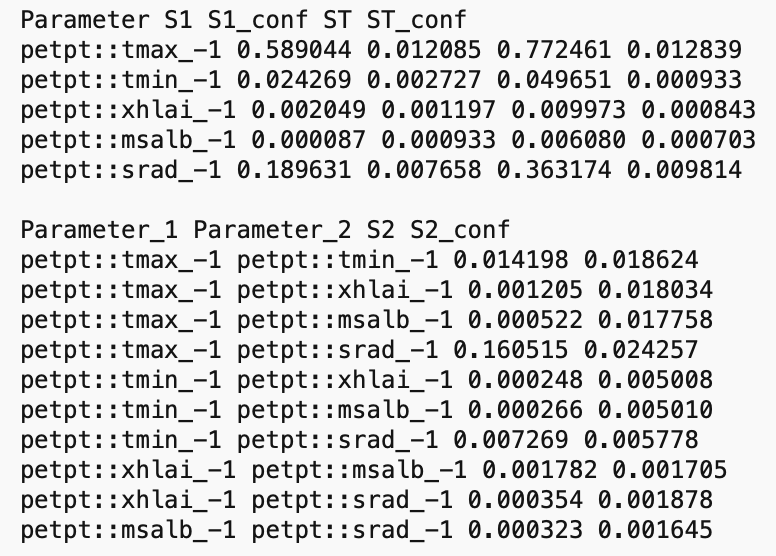
\includegraphics[width=.8\columnwidth]{sensitivity_indices}%
    \caption[PETPT Sensitivity Indices]{An example of all of the sensitivity indices returned by SALib for the PETPT evapo-transpiration model. This set of indices was created from a sample set of $50,000$ input samples for the PETPT model.}
\end{figure}
\FloatBarrier

In the figure we see that the $S_1$, $S_2$, and $S_T$ sensitivity indices are all computed and returned by this method of Sobol analysis as well as the $95\%$ confidence interval bounds for each value of each index.
We know that the ordered sensitivity indices computed using this method will sum to $1$ if all of the higher order indices are present \citep{sobol2001globalSA}.
We also know that the larger the value for any sensitivity index, the more of an affect the uncertainty in the corresponding input or set of inputs has on the uncertainty in model output.
Therefore we can use this information to inform our decisions about the model based on the uncertainty caused from model inputs.
For example, we can see that for the PETPT model, over $95\%$ of the uncertainty in the output of the model is caused by single or double variable interactions.
Not only is it very useful to have a scaled representation of causal uncertainty represent with each set of inputs, but the uniform scaling also allows for comparisons of scale across the inputs of multiple competing scientific models.

The total order index $S_T$ is also useful for decision making amongst our scientific models.
While this index does not sum to $1$ for the set of inputs, it is guaranteed to be greater than or equal to one, and allows us to see which input has the greatest compounded affect on output uncertainty.
We can use this information across models as well.
While we cannot compare scales across models without a normalizing factor, we can easily produce categorical comparisons across models of which inputs have the highest total order affects.

In the following sections of this chapter several use cases of the sensitivity indices will be presented.
However, the Sobol analysis method also returns useful information about the confidence in the estimate for each sensitivity index.
This information can be used to empirically determine if enough samples were included for the analysis to be successful.
A simple metric to use for this purpose is to have a cutoff for the largest confidence interval size.
If a confidence interval is returned that is larger than that maximum size, then add more samples from the Sobol sequence and rerun the analysis phase.
The SMS pipeline includes the usage of this technique to ensure that the sensitivity indices being used for analysis are sufficiently descriptive of the competing models.

\subsection{Model Output Surface\label{sec:out_surf}}
Although the sensitivity indices for a given scientific model are able to provide information on what input variables cause the most uncertainty upon the model output they do not provide any information about how the model output varies as a set of input variables varies.
However, this information is likely valuable to modelers as it will aid in their ability to distinguish between models based on the functional form of their outputs as a function of the most variable inputs.
To accomplish this goal, I created a new method that creates a plot of the output variable as a function of the two most sensitive inputs based upon the results from sensitivity analysis.
I refer to these new plots as a Model Output Surface (MOS) plot.

A MOS plot is a 3D plot where the z-axis is the output variable of a model and the remaining axes are input variables.
A MOS plot consists of the plotted outputs over a predefined range for each of the two inputs which creates a smooth surface object in three dimensions.
Evaluation to create this surface is done using a mesh grid of finite points.
Extrapolation between point evaluations can then be conducted to create the smooth surface visualization.
As expected, a higher number of input samples over the same input space range will lead to a smoother surface that is a more accurate representation of the true output surface for the input pair.
In this section I will cover the process of selecting which input variables to study with MOS plots, how to set values for the additional inputs not under study, and how to efficiently perform the evaluations necessary to generate a MOS plot.

\subsubsection{Input Variable Selection\label{sec:inp_var_sel}}
Most models will have more than two input variables and thus when creating a MOS plot a decision must be made about which two input variables should be varied during output surface creation. Generally speaking, for a model with $N$ input variables, a user could generate $\frac{N(N+1)}{2}$ plots to expose all possible pairs of variable interactions and examine how those interactions affect the output surface. For most sizes of $N$ this study is likely to not be computationally feasible, and modelers are unlikely to desire to view such a large number of output plots when performing model selection. A better use-case for MOS plots would be to showcase the pairs of variables that have the greatest combined affect on the model output.

In order to accomplish this task we need a way to rank the pairs of inputs in order of how greatly they affect model output. Fortunately we can attain this ranking directly from the second order sensitivity index, $S_2$. Utilizing the $S_2$ index as our ranking schema we can either create MOS plots for the top $k$ variable pairs, or we can use a threshold cutoff and create MOS plots for all pairs on input variables that exceed this cutoff. An appropriate cutoff could be a pre-defined value, or it could be based upon a difference between neighboring values of the sorted $S_2$ indices. An example of such a cutoff would be to generate MOS plots for all input pairs, until seeing a drop in $S_2$ index score of at least an order of magnitude.

It is important to note that utilizing the $S_2$ index is not the only way to select which input pairs to generate a MOS plot for, and is likely not the only metric of interest to modelers. If we have additional information, such as which inputs can be most or least accurately measured by the modelers then we may want to generate MOS plots for the modelers based upon this criterion so they can observe how output varies for input variables that they can measure well, vs those that they can measure poorly. This will becomes more important for model selection when competing models have differing sets of inputs, some of which may be easier or harder to measure than others.

\subsubsection{Input parameter estimation\label{sec:inp_param_est}}
Once the input variables for a given MOS plot are selected, the remaining inputs must have values assigned to them to allow for the model to be evaluated for MOS plot generation. To avoid confusion, I will refer to this set of input variables that will no longer be varied as the input parameters for the model.

There are many options present for assigning values to each of the input parameters. Unfortunately the nature of models also demands that either one or few values be chosen for each of the input parameters due to the high number of input parameters that are likely to be present. Even if we wished to allow for only two values for each input parameter, and wanted to study all possible combinations of them then for a set of $N$ input parameters we would generate $2^N$ MOS plots. Expecting modelers to review this many MOS plots goes against the idea of summarizing model behavior. This entails that a single set of values for the input parameters should be selected.

The task of input parameter estimation is now the task of finding the best-fit set of input parameters for a MOS plot. For each parameter we know that we have a range of values that were used for the parameter during analysis. From this information we can define that the best-fit for an input parameter is the Maximum Likelihood Estimate (MLE) over the range. The MLE is a useful estimate for each input parameter since the ranges are included for each parameter. However, if observational data were present, then it would be possible to use the Maximum A Priori (MAP) estimate as the setting for our input parameters.

\subsubsection{Surface Generation and Evaluation\label{sec:surf_usage}}
Once the decisions for the input variables to study and the preset parameter values to use have been made a MOS plot is easy to generate.
Generation requires model evaluation over large numbers of sets of inputs.
Since the plot itself takes the form of a meshgrid the amount of required evaluations will scale as expected for a meshgrid structure.
This means that if we want to study $1,000$ examples of each of the two variables under study we will need $1,000,000$ total evaluations.
Luckily this computation can be done efficiently using PyTorch tensor computation.
Once the evaluations are completed a MOS plot can be easily rendered and will appear interactively for the modelers. Below is an example of a MOS plot that would be presented for a modeler interested in working with the PETPT evapo-transpiration model.

\FloatBarrier
\begin{figure}[!htbp]
    \label{mos_plot_ex}
    \centering
    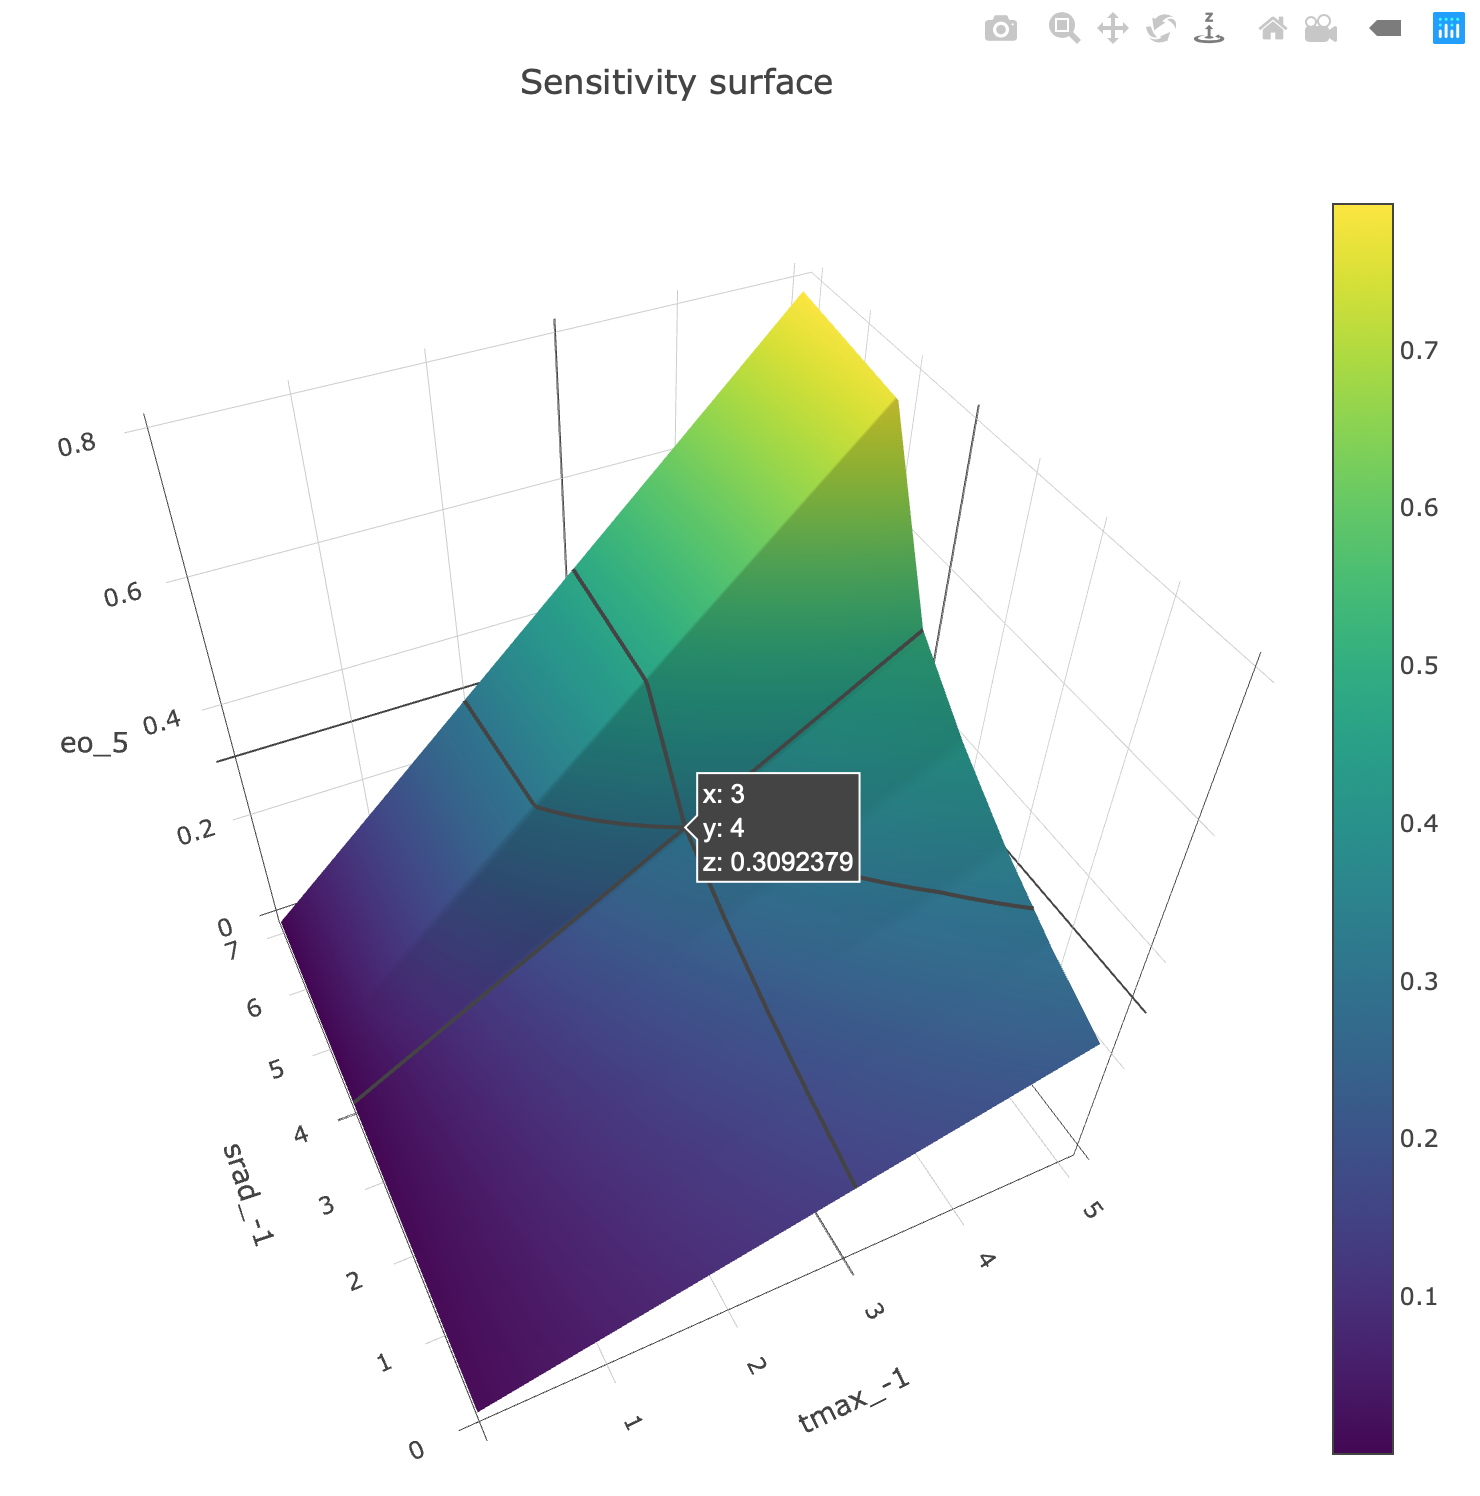
\includegraphics[width=.8\columnwidth]{sensitivity_surface}%
    \caption[PETPT Example MOS Plot]{An example of a MOS plot for the PETPT evapo-transpiration model. In this plot the two variables under study are solar radiation and the maximum temperature. Notice that these two variables covary and their variance greatly affects the shape of the model output surface.}
\end{figure}
\FloatBarrier

\subsection{Model Report Generation\label{sec:report_gen}}
Utilizing the information provided by the sensitivity indices of a model allows the SMS pipeline to gain insight about how the uncertainty in the output of the model is caused by the various inputs of the model.
However, this information alone is likely still too opaque to be useful to modelers when selecting a model for an experiment.
Ultimately the task of model selection comes down to an optimization problem for modelers based upon the desires they have for a models performance.
These tasks will likely differ between different modelers, but will almost certainly have some common themes.
In order to make the SMS pipeline as useful as possible to modelers we seek to provide modelers with the direct information from the sensitivity indices and also to provide them with useful abstractions created from the sensitivity indices that further differentiate competing models.
In this section I define the information contained in a model report that aims to differentiate two models so that modelers can perform their own model selection.

\subsubsection{Minimizing Measurement Error\label{sec:min_measure_error}}
When a modeler uses a model in an experiment they will need some method of collecting data for the inputs.
In almost all cases this immediately requires a modelers to address the question of: "how confident are you in your ability to measure input phenomena $x$?"
A modeler will likely want to select a model whose output is least sensitive to errors in measurements from the inputs that they are least able to measure accurately.
Only the modeler is aware of the measurement error associated with the devices used to measure each of their inputs; however, the information recovered in the sensitivity indices can be combined with the measurement error of each input to give the modeler a clear view of which model will perform best for them based upon minimizing the impact of measurement error.
Therefore, providing the sensitivity index information in an interpretable table as part of the model report is crucial for modelers.

\subsubsection{Cross-model Output Surface Examination \label{sec:multi_mod_surface}}
The sensitivity indices give a clear picture of which inputs or sets of inputs contribute the greatest amount of uncertainty to the model output.
Comparing sensitivity indices across the shared inputs of multiple models allows us to see where different models have the greatest amount of uncertainty.
However, this is still a summary statistic of the variance in model output caused by variance in the inputs.
While summary statistics are sufficient for some use cases, many modelers will likely want to base their model selection decision on the differences in shape of the model output for key variables that are shared between competing models.

This information can be provided to the modelers by the SMS pipeline in the form of comparative MOS plots, one per model, for given pairs of shared input variables that are of interest to the modelers.
These comparative MOS plots allow modelers to diagnose the functional differences in how two models differ based upon each individual models input variables of highest sensitivity, or based upon a shared set of input variables that have the highest combined sensitivity between the two models.
Modelers would be able to observe these surfaces without the aid of the SMS pipeline; however, without the information extracted from sensitivity analysis during the SMS pipeline modelers would need to generate MOS plots for every possibly set of input pairs.
The SMS pipeline removes this burden upon modelers by discovering which pairs of inputs are the most crucial to focus upon and automatically presenting those to modelers so that they can make expedient decisions amongst competing scientific models.
